
\chapter{Premier apprentissage automatique : Régression Linéaire}

\section{Codage de la Régression Lineaire manuelle}
Il s'agit du problème classique de régression linéaire. on se donne un ensemble de valeurs de $x$, et un ensemble de valeurs attendues pour chacun de ces $x$. L'objectif est de trouver la droite qui passe le plus près de tous ces points.
\begin{mypython}
import tensorflow as tf

x = tf.placeholder(tf.float32)
sortieVoulue = tf.placeholder(tf.float32)

W = tf.Variable([.3], dtype=tf.float32)
b = tf.Variable([-.3], dtype=tf.float32)

sortieCalculee = W*x + b
\end{mypython}
Nous avons bien défini nos entrées :
\begin{itemize}
\item $x$ : un placeholder dans lequel nous placerons au moment du run les abscisses des points
\item $y$ : un placeholder dans lequel nous placerons au moment du run les ordonnées des points
\end{itemize}

Par ailleurs, nous allons chercher des droites, qui sont paramétrées par leur pente $W$ et leur abscisse à l'origine $b$. Nous avons fixé les valeurs initiales de $W$ et $b$ a respectivement 0.3 et -0.3. Pour un couple $(W,b)$, nous avons une droite qui à $x$ associe $sortieCalculee$.
Notre problème consiste donc a modifier $W$ et $b$ pour que $sortieCalculee$ soit aussi prêt que possible de $sortieVoulue$.
Pour un couple $(W,b)$, évaluons l'erreur que l'on commet. on peut mesurer la somme des erreurs quadratiques sur chaque entrée :

\begin{mypython}
squared_deltas = tf.square(sortieCalculee - sortieVoulue)
erreur = tf.reduce_sum(squared_deltas)
\end{mypython}
Ajoutons enfin le run qui permettra de faire ces calculs pour les valeurs initiales de W et b :
\begin{mypython}
sess = tf.Session()

init = tf.global_variables_initializer()
sess.run(init)

print("erreur :",sess.run(erreur,{x: [1, 2, 3, 4], sortieVoulue: [0, -1, -2, -3]}))
\end{mypython}
Pour nos valeurs initiales, l'erreur totale est donnée par la sortie suivante
\begin{myoutput}
erreur : 23.66
\end{myoutput}
De fait, quelques calculs rapides permettrait de trouver les meilleures valeurs possible de W,b : (-1, 1). Dans le cas particulier des x et sortieVoulue donnés, il existe réellement une droite qui passe par ces points...

Essayons de vérifier cela 
\begin{mypython}
fixW = tf.assign(W, [-1.])
fixb = tf.assign(b, [1.])
sess.run([fixW, fixb])

print("erreur :",sess.run(erreur,{x: [1, 2, 3, 4], sortieVoulue: [0, -1, -2, -3]}))
\end{mypython}
Les deux premières lignes créent chacune un noeud dont l'objectif est de corriger les valeurs de $W$ et $b$. La troisième ligne lance le calcul sur ces nœuds, modifiant ainsi les valeurs de nos variables
Enfin la dernière ligne calcule l'erreur pour les $x$ et $sortieVoulue$ fournis avec le résultat suivant :
\begin{myoutput}
erreur : 0.0
\end{myoutput}
Essayons maintenant de trouver automatiquement ces valeurs pour W et b :
\begin{mypython}
optimizer = tf.train.GradientDescentOptimizer(0.01)
train = optimizer.minimize(erreur)

sess.run(init) # reset values to incorrect defaults.
for i in range(1000):
  sess.run(train, {x: [1, 2, 3, 4], sortieVoulue: [0, -1, -2, -3]})

print("(W,b finaux) :", sess.run([W, b]))
\end{mypython}
Pour cela, nous utilisons un objet \textbf{optimizer} prédéfini par TensorFlow, et qui opérera une descente de gradient (avec un pas de 0.0.1). On définit un nœud de calcul (train) dont le but est de minimiser  l'erreur.
La ligne suivante réinitialise les valeurs de $W$ et $b$ à (0.3, -0.3)
puis, 1000 fois de suite, on calcule le nœud train. Chaque itération améliore un peu les valeurs $(W et b)$. Il faut noter que nulle part, on ne spécifie que les valeurs à modifier sont $W$ et $b$... le programme le devine à partir du graphe : $W$ et $b$ sont les seules variables du graphe....
Enfin la dernière ligne affiche les valeurs finales trouvées :
\begin{myoutput}
(W,b finaux):[array([-0.9999969], dtype=float32), array([0.9999908], dtype=float32)]
\end{myoutput}

On voit que notre programme a trouvé pour $W$ et $b$ des valeurs très proches des valeurs cherchées (-1,1)
Voici donc le code du programme complet. Ce code est contenu dans le fichier :\\
\verb+DNN/Documentation/TutosPython/RegressionLineaire/regressionLineaire.py+

\lstinputlisting[style=generalFrame,backgroundcolor=\color{darkwhite}]{../../TutosPython/RegressionLineaire/regressionLineaire.py}

Voici également le graphe de calcul que notre programme a utilisé
\begin{figure}[H]

\begin{center}
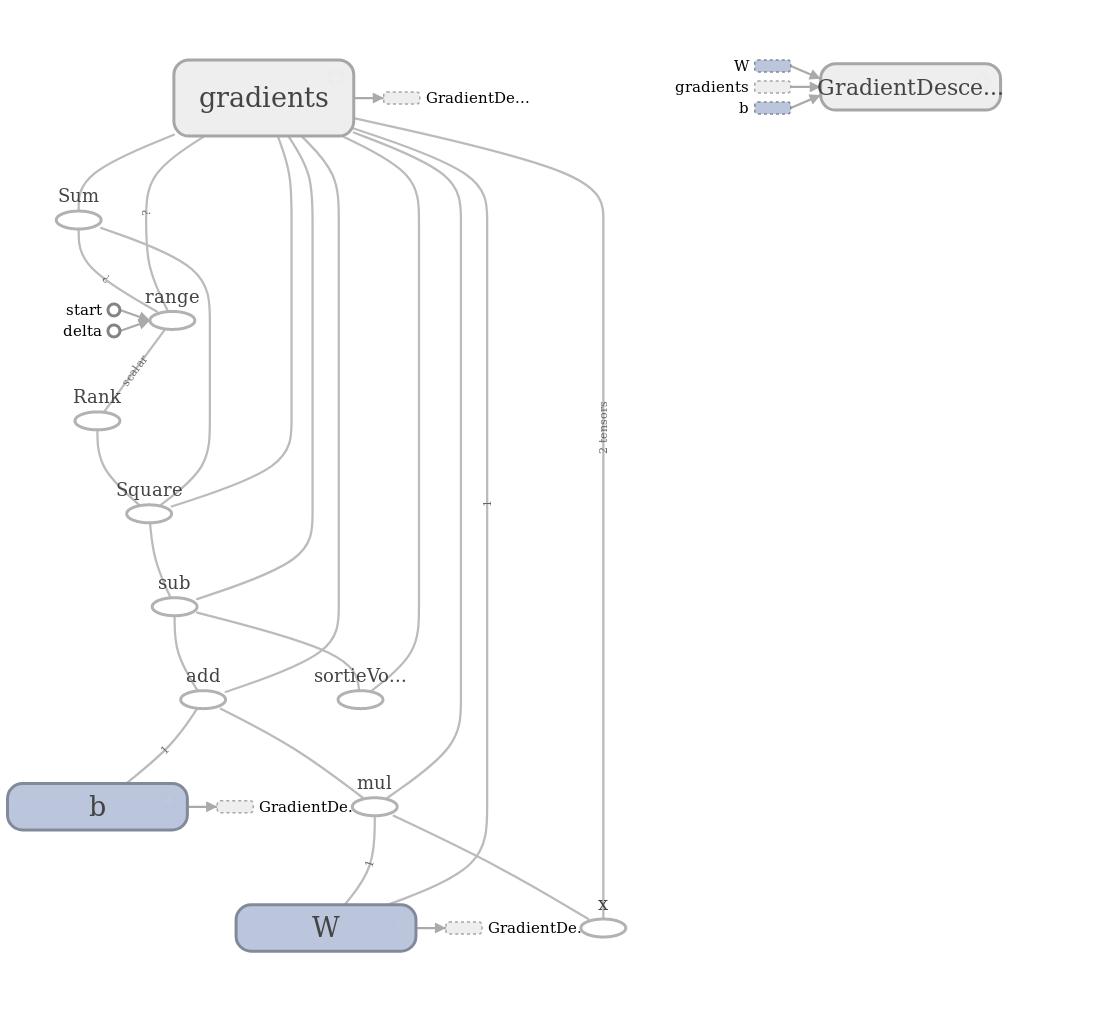
\includegraphics[width=10cm]{./figures/graphRegressionLineaire.png} 
\end{center}
\caption{Graphe de calcul pour la régression linéaire}
\end{figure}

En l'état, une partie de ce graphe est facile a expliquer (en bas a gauche), le reste est assez... mystérieux mais est clairement associé a la descente du gradient...

\section{Suivi de performance dans TensorBoard}
Nous voulons suivre l’évolution de l'erreur au cours de l'apprentissage des $W$,$b$ du programme précédent et la visualiser à l'aide de TensorBoard.
Il va falloir modifier notre programme TensorFlow pour logger cette erreur. Les lignes à insérer étant réparties un peu partout, nous indiquerons chaque modification séparément et fourniront le code complet en fin de section.

Tout d'abord, il faut signaler que l'on s'intéresse à l'erreur. Ceci est fait par la ligne suivante :
\begin{mypython}
tf.summary.scalar('erreur quadratique', erreur)
\end{mypython}
De ce que nous avons compris, on peut s’intéresser à plusieurs paramètres, et il faudra les fusionner pour les logger avec la ligne suivante :
\begin{mypython}
merged = tf.summary.merge_all()
\end{mypython}
Lors de chaque run, pendant l’entraînement, il faudra demander le calcul de ce merged. Enfin, le résumé devra être sauvé grâce au writer de TensorBoard... 
\begin{mypython}
for i in range(1000):
  summary, _ = sess.run([merged,train], {x: [1, 2, 3, 4], sortieVoulue: [0, -1, -2, -3]})
  writer.add_summary(summary, i)
\end{mypython}
Si une partie des notions utilisées ici nous échappe, voici néanmoins le code du programme complet. Ce code est contenu dans le fichier :\\
\verb+DNN/Documentation/TutosPython/RegressionLineaire/regressionLineaireTensorBoard.py+

\lstinputlisting[style=generalFrame,backgroundcolor=\color{darkwhite}]{../../TutosPython/RegressionLineaire/regressionLineaireTensorBoard.py}

Voici le résultat final visualisé dans TensorBoard
\begin{figure}[H]

\begin{center}
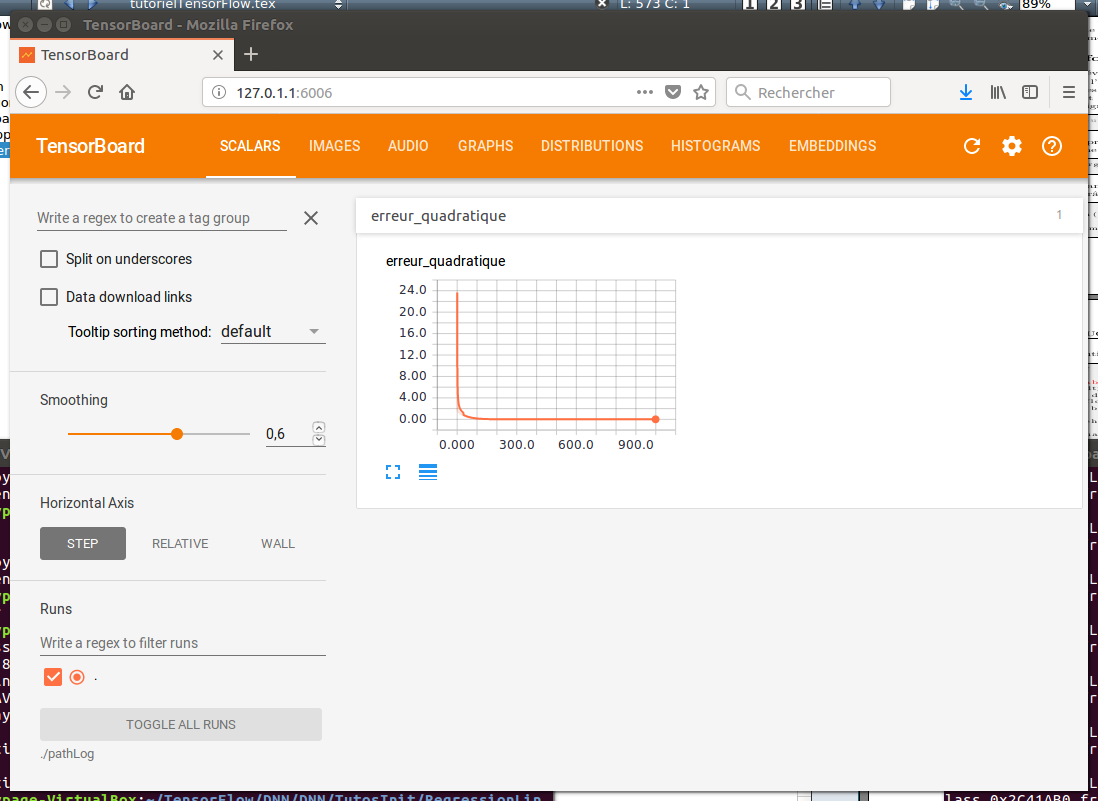
\includegraphics[width=10cm]{./figures/TBScalarRegression.png} 
\end{center}
\caption{Visualisation de l'évolution de l'erreur lors de l'apprentissage}
\end{figure}

\section{Régression Linéaire avec Estimator}

Estimator est une bibliothèque TensorFlow de haut niveau qui simplifie la mécanique de l'apprentissage automatique, notamment:
\begin{itemize}
\item exécuter des boucles d'entraînement
\item exécuter des boucles d'évaluation
\item gérer des ensembles de données
\end{itemize}

Estimator définit de nombreux modèles courants.
Utilisons le ici pour le problème précédent de régression linéaire
\begin{mypython}
# NumPy is often used to load, manipulate and preprocess data.
import numpy as np
import tensorflow as tf

# Declare list of features. We only have one numeric feature. There are many
# other types of columns that are more complicated and useful.
feature_columns = [tf.feature_column.numeric_column("x", shape=[1])]

# An estimator is the front end to invoke training (fitting) and evaluation
# (inference). There are many predefined types like linear regression,
# linear classification, and many neural network classifiers and regressors.
# The following code provides an estimator that does linear regression.
estimator = tf.estimator.LinearRegressor(feature_columns=feature_columns)

# TensorFlow provides many helper methods to read and set up data sets.
# Here we use two data sets: one for training and one for evaluation
# We have to tell the function how many batches
# of data (num_epochs) we want and how big each batch should be.
x_train = np.array([1., 2., 3., 4.])
y_train = np.array([0., -1., -2., -3.])
x_eval = np.array([2., 5., 8., 1.])
y_eval = np.array([-1.01, -4.1, -7, 0.])

input_fn = tf.estimator.inputs.numpy_input_fn(
    {"x": x_train}, y_train, batch_size=4, num_epochs=None, shuffle=True)

train_input_fn = tf.estimator.inputs.numpy_input_fn(
    {"x": x_train}, y_train, batch_size=4, num_epochs=1000, shuffle=False)

eval_input_fn = tf.estimator.inputs.numpy_input_fn(
    {"x": x_eval}, y_eval, batch_size=4, num_epochs=1000, shuffle=False)

# We can invoke 1000 training steps by invoking the  method and passing the
# training data set.
estimator.train(input_fn=input_fn, steps=1000)

# Here we evaluate how well our model did.
train_metrics = estimator.evaluate(input_fn=train_input_fn)
eval_metrics = estimator.evaluate(input_fn=eval_input_fn)

print("train metrics: %r"% train_metrics)
print("eval metrics: %r"% eval_metrics)
\end{mypython}

Le code est relativement simple. On peut noter que :
\begin{itemize}
\item on ne construit plus le graphe nous même
\item On ne lance plus de run manuellement. Tout ceci est fait dans les fonctions train et evaluate.
\end{itemize}

\section{Régression Linéaire avec un modèle personnalisé pour Estimator}
Estimator ne vous verrouille pas dans ses modèles prédéfinis. Supposons que nous voulions créer un modèle personnalisé qui n'est pas intégré dans TensorFlow, en conservant  l'abstraction de haut niveau de jeu de données, l' alimentation, la formation, etc. de Estimator. Içi, nous allons implémenter notre propre modèle équivalent au LinearRegressor.
Pour définir un modèle personnalisé qui fonctionne avec Estimator, nous devons utiliser \verb+tf.estimator.Estimator+.  Nous fournissons simplement à Estimator une fonction \verb+model_fn+ qui indique à Estimator comment il peut évaluer les prédictions, les étapes d'entraînement et la perte. voici néanmoins le code du programme complet. Ce code est contenu dans le fichier :\\
\verb+DNN/Documentation/TutosPython/RegressionLineaire/regressionLineaireTfEstimatorPerso.py+

\lstinputlisting[style=generalFrame,backgroundcolor=\color{darkwhite}]{../../TutosPython/RegressionLineaire/regressionLineaireTfEstimatorPerso.py}
